\documentclass[aspectratio=169]{beamer}
\usepackage[T1]{fontenc}
\usepackage[utf8]{inputenc}
\usepackage{listings}
\usepackage{colortbl}

\definecolor{codegreen}{rgb}{0,0.6,0}
\definecolor{codegray}{rgb}{0.5,0.5,0.5}
\definecolor{codepurple}{rgb}{0.58,0,0.82}
\definecolor{backcolour}{rgb}{0.95,0.95,0.92}

\lstdefinestyle{mystyle}{
    backgroundcolor=\color{backcolour},
    commentstyle=\color{codegreen},
    keywordstyle=\color{magenta},
    numberstyle=\tiny\color{codegray},
    stringstyle=\color{codepurple},
    basicstyle=\ttfamily\footnotesize,
    breakatwhitespace=false,
    breaklines=false,
    captionpos=b,
    keepspaces=true,
    numbers=left,
    numbersep=5pt,
    showspaces=false,
    showstringspaces=false,
    showtabs=false,
    tabsize=2
}

\lstdefinestyle{yaml}{
    basicstyle=\color{blue}\footnotesize,
    string=[s]{'}{'},
    comment=[l]{:},
    morecomment=[l]{\-},
    backgroundcolor=\color{backcolour},
    commentstyle=\color{codegreen},
    keywordstyle=\color{magenta},
    numberstyle=\tiny\color{codegray},
    stringstyle=\color{codepurple},
    basicstyle=\ttfamily\footnotesize,
    breakatwhitespace=false,
    breaklines=false,
    captionpos=b,
    keepspaces=true,
    numbers=left,
    numbersep=5pt,
    showspaces=false,
    showstringspaces=false,
    showtabs=false,
    tabsize=2
 }

\lstdefinestyle{ww}{
    basicstyle=\color{blue}\footnotesize,
    morestring=[b]{"},
    comment=[s]{.}{\ },
    morecomment=[s]{.}{\}},
    morecomment=[s]{\$}{\ },
    morecomment=[s]{\$}{\}},
    backgroundcolor=\color{backcolour},
    commentstyle=\color{codegreen},
    keywordstyle=\color{magenta},
    numberstyle=\tiny\color{codegray},
    stringstyle=\color{codegreen},
    basicstyle=\ttfamily\footnotesize,
    breakatwhitespace=false,
    breaklines=false,
    captionpos=t,
    keepspaces=true,
    numbers=left,
    numbersep=5pt,
    showspaces=false,
    showstringspaces=false,
    showtabs=false,
    tabsize=2,
    keywords={if,range,end},
 }

\lstdefinestyle{wwctl}{
    language=bash,
    basicstyle=\color{blue}\footnotesize,
    backgroundcolor=\color{backcolour},
    commentstyle=\color{codegreen},
    keywordstyle=\color{magenta},
    numberstyle=\tiny\color{codegray},
    stringstyle=\color{codegreen},
    basicstyle=\ttfamily\footnotesize,
    breakatwhitespace=false,
    breaklines=true,
    captionpos=t,
    keepspaces=true,
    numbers=left,
    numbersep=5pt,
    showspaces=false,
    showstringspaces=false,
    showtabs=false,
    tabsize=2,
    morestring=[s]{\ W}{=},
    keywords={wwctl,container,import,shell,export,node,add,set,list},
 }



\lstset{style=mystyle}

\title{warewulf\\
making cluster\\
installations fast and \\
reliable}
\date{April 25, Ostrava}
\author{Christian Goll <\texttt{cgoll@suse.com}>}
\usetheme{suse}

\begin{document}

\begin{frame}
\titlepage
\end{frame}
\begin{frame}[fragile]
\frametitle{Introduction}
\framesubtitle{warewulf is tool for managing beowulf clusters}
\begin{columns}
\column{0.5\textwidth}
\begin{block}{Beowulf}
  \begin{itemize}
    \item old british poem
  \end{itemize}
\end{block}
\begin{block}{Beowulf cluster}
  \begin{itemize}
    \item became popular in the 90.
    \item use of the shelf hardware
    \begin{itemize}
      \item 486 \& linux
      \item \textbf{not} Cray \& unix
    \end{itemize}
    \item warewulf is a typo of werewolf
  \end{itemize}
\end{block}
\column{0.5\textwidth}
  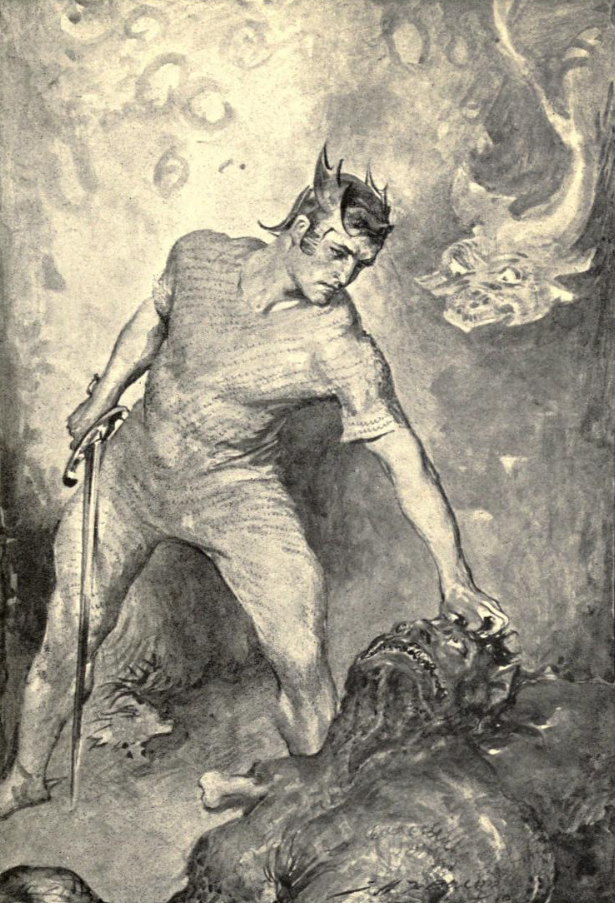
\includegraphics[width=.6\linewidth]{Beowulf}
\end{columns}
\end{frame}

\begin{frame}[fragile]
\frametitle{Introduction}
\framesubtitle{HPC landscape}
\begin{block}{Top five Supercomputers}
\begin{table}
\begin{tabular}{c|l|l|l|l}
1 &	Frontier& EPYC 64C &AMD MI250X &Slingshot-11 \\
2 &	Aurora  & Xeon 9470 & Intel GPU Max&Slingshot-11 \\
3 &	Eagle & Xeon 8480 &  NVIDIA H100 & NVIDIA Infiniband \\
\rowcolor{backcolour}
4 &	Fugaku &  A64FX 48C 2.2GHz & - & Tofu interconnect D \\
5 &	LUMI &  EPYC 64C 2GHz & AMD MI250X & Slingshot-11 
\end{tabular}
\end{table}
\begin{itemize}
  \item only Fugaku uses non standard CPU
  \item others are beowulf clusters with GPUs attached
\end{itemize}
\end{block}
\end{frame}
\begin{frame}[fragile]
\frametitle{Introduction}
\framesubtitle{Beowulf cluster}
\begin{columns}
\column{0.5\textwidth}
\begin{block}{base components}
\begin{itemize}
  \item management node
  \item compute nodes
  \item management network
\end{itemize}
\end{block}
\begin{block}{optional components}
\begin{itemize}
  \item more compute nodes
  \item fast network interconnects 
  \item central storage
  \item bmc/ipmi
\end{itemize}
\end{block}
\column{0.5\textwidth}
  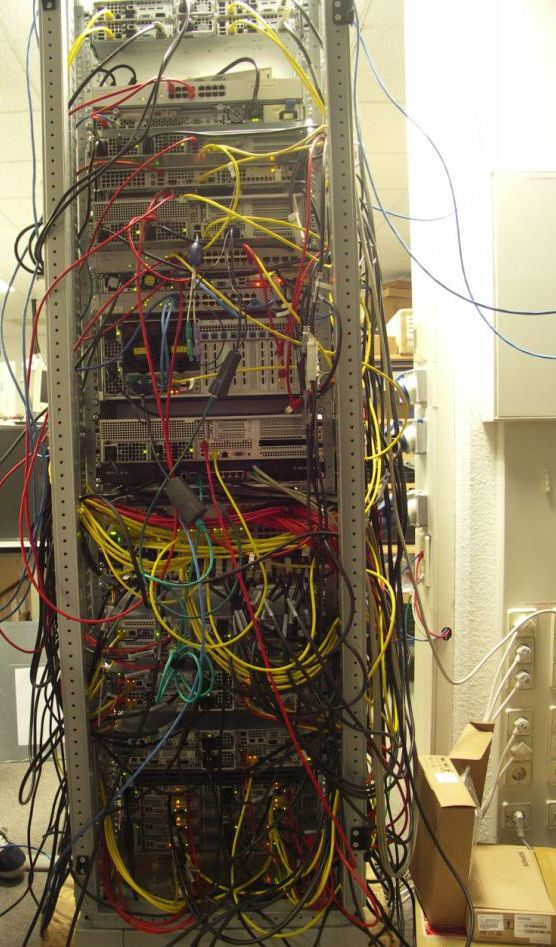
\includegraphics[width=.6\linewidth]{Transtec-056}
\end{columns}
\end{frame}
\begin{frame}[fragile]
\frametitle{Introduction}
\framesubtitle{Beowulf Cluster}
\begin{columns}
\column{0.5\textwidth}
\begin{block}{differences to data centers}
  \begin{itemize}
    \item compute nodes are cattle
    \item hierarchical organization
    \item compute are not updated after boot process
    \item application come from central storage
    \item applications are self compiled
    \item one application can run over several nodes
  \end{itemize}
\end{block}
\column{0.5\textwidth}
  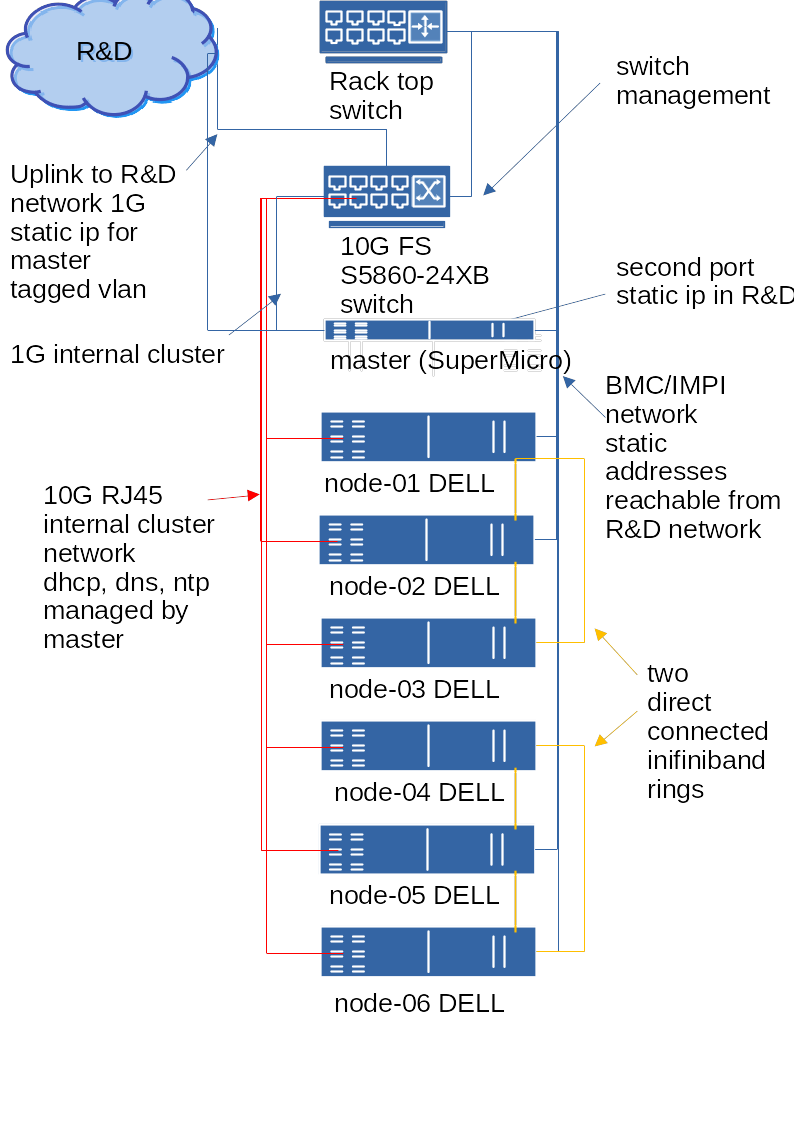
\includegraphics[width=.6\linewidth]{networkplan}
\end{columns}
\end{frame}
\begin{frame}[fragile]
\frametitle{Warewulf description}
\framesubtitle{software stack}
\begin{columns}
\column{0.5\textwidth}
  \begin{block}{warewulf components}
  \hspace*{.1\linewidth}\begin{minipage}{.8\linewidth}
  \begin{block}{warewulfd delivers}
    \begin{itemize}
      \item kernel \& modules
      \item node image
      \item node configurations
    \end{itemize}
  \end{block}
  \begin{block}{\texttt{wwctl} cmd line tool}
    \begin{itemize}
      \item manages node database
      \item manages node image
    \end{itemize}
  \end{block}
  \vspace*{1cm}
  \end{minipage}
  \end{block}
\column{0.5\textwidth}
  \begin{block}{external components}
  \hspace*{.1\linewidth}\begin{minipage}{.8\linewidth}
    \begin{block}{dhcp server}
      \begin{itemize}
      \item ISC dhcpd server
      \item dnsmasq
    \end{itemize}
    \end{block}
    \begin{block}{tftp}
      \begin{itemize}
      \item tftp from \texttt{kernel.org}
      \item dnsmasq
    \end{itemize}
    \end{block}
  \end{minipage} 
  \end{block}
  \begin{block}{optional}
    \begin{itemize}
      \item nfs
      \item manage \texttt{/etc/hosts}
    \end{itemize}
  \end{block}
\end{columns}
\end{frame}

\begin{frame}[fragile]
\frametitle{Warewulf configuration}
\framesubtitle{database \texttt{/etc/warewulf/nodes.conf}}
\begin{columns}
\column{0.5\textwidth}
\begin{itemize}
  \item plain yaml file
  \item easy backup
  \item can be version controlled
  \item external tools support
  \begin{itemize}
    \item vim, ansible
  \end{itemize}
\end{itemize}
\begin{block}{profiles}
\begin{itemize}
  \item stores identical values for collection of nodes
  \item values can be overridden on node basis
\end{itemize}
\end{block}
\column{0.5\textwidth}
\begin{lstlisting}[style=yaml]
WW_INTERNAL: 45
nodeprofiles:
  default:
    comment: This profile is automatically included for each node
    container name: leap
    network devices:
      default:
        device: eth0
nodes:
  n01:
    profiles:
    - default
    network devices:
      default:
        hwaddr: 52:54:00:4e:cb:1d
        ipaddr: 172.16.130.101
  n02:
\end{lstlisting}
%
\end{columns}
\end{frame}
\begin{frame}[fragile]
\frametitle{Warewulf configuration}
\framesubtitle{command line database manipulation}
\begin{columns}
\column{0.25\textwidth}
\begin{block}{add node}
\begin{lstlisting}[style=wwctl]
wwctl node add n01 -I 10.10.10.1
\end{lstlisting}
\end{block}
\begin{block}{modify node}
\begin{lstlisting}[style=wwctl]
wwctl node set n01 --comment "Have fun"
\end{lstlisting}
\end{block}
\begin{block}{list node}
\begin{lstlisting}[style=wwctl]
wwctl node list n01 -a
\end{lstlisting}
\end{block}
\vspace*{3cm}
\column{0.75\textwidth}
\begin{lstlisting}[style=mystyle]
NODE FIELD                    PROFILE    VALUE
n01  Id                       --         n01
n01  Comment                  SUPERSEDED Have fun
n01  ContainerName            default    leap
n01  Ipxe                     --         (default)
n01  RuntimeOverlay           --         (generic)
n01  SystemOverlay            --         (wwinit)
n01  Root                     --         (initramfs)
n01  Discoverable             --         false
n01  Init                     --         (/sbin/init)
n01  Kernel.Args              --         (quiet crashkernel=no vga=791 net.naming-scheme=v238)
n01  Profiles                 --         default
n01  PrimaryNetDev            --         (default)
n01  NetDevs[default].Type    --         (ethernet)
n01  NetDevs[default].OnBoot  --         (true)
n01  NetDevs[default].Device  default    eth0
n01  NetDevs[default].Hwaddr  --         52:54:00:4e:cb:1d
n01  NetDevs[default].Ipaddr  --         172.16.130.101
n01  NetDevs[default].Netmask --         (255.255.255.0)
n01  NetDevs[default].Primary --         (true)
\end{lstlisting}
\end{columns}
\end{frame}
\begin{frame}[fragile]
\frametitle{Warewulf configuration}
\framesubtitle{templates\& overlays}
\begin{columns}
\column{0.5\textwidth}
\begin{block}{Configuration templates}
  \begin{itemize}
    \item based on go templates
    \item $\{\{ .foo \}\}$ replaced \\
    with variable \texttt{foo}
    \item exported go function \\
    can be called
  \end{itemize}
\end{block}
\begin{block}{Configuration overlays}
\begin{itemize}
  \item rendered templates packed\\
  into overlay
  \item overlay put ontop \\
  of node image
\end{itemize}
\end{block}
\column{0.5\textwidth}
\begin{lstlisting}[style=ww,caption=/etc/issue.ww]
Warewulf Node:      {{.Id}}
Container:          {{.Container}}
{{ if .Kernel.Version }}Kernel:             {{.Kernel.Version}} {{ end -}}
Kernelargs:         {{.Kernel.Args}}

Network:
{{- range $devname, $netdev := .NetDevs}}
    {{$devname}}: {{$netdev.Device}}
    {{$devname}}: {{$netdev.IpCIDR}}
{{if $netdev.Ipaddr6 }}    {{$devname}}: {{$netdev.Ipaddr6}}{{ end -}}
{{if $netdev.Hwaddr }}    {{$devname}}: {{$netdev.Hwaddr}}{{ end -}}
{{end}}
\end{lstlisting}
\end{columns}
\end{frame}
\begin{frame}[fragile]
\frametitle{Warewulf configuration}
\framesubtitle{rendered templates}
\begin{columns}
\column{0.5\textwidth}
\begin{block}{Configuration templates}
  \begin{itemize}
    \item based on go templates
    \item $\{\{ .foo \}\}$ replaced \\
    with variable \texttt{foo}
    \item exported go function \\
    can be called
  \end{itemize}
\end{block}
\begin{block}{Configuration overlays}
\begin{itemize}
  \item rendered templates packed\\
  into overlay
  \item overlay put ontop \\
  of node image
\end{itemize}
\end{block}
\column{0.5\textwidth}
\begin{lstlisting}[style=ww,caption=/etc/issue.ww]
Warewulf Node:      {{.Id}}
Container:          {{.Container}}
{{ if .Kernel.Version }}Kernel:             {{.Kernel.Version}} {{ end -}}
Kernelargs:         {{.Kernel.Args}}

Network:
{{- range $devname, $netdev := .NetDevs}}
    {{$devname}}: {{$netdev.Device}}
    {{$devname}}: {{$netdev.IpCIDR}}
{{if $netdev.Ipaddr6 }}    {{$devname}}: {{$netdev.Ipaddr6}}{{ end -}}
{{if $netdev.Hwaddr }}    {{$devname}}: {{$netdev.Hwaddr}}{{ end -}}
{{end}}
\end{lstlisting}
\end{columns}
\end{frame}
\begin{frame}[fragile]
\frametitle{Warewulf configuration}
\framesubtitle{overlays}
warewulf defines two types of overlays
\begin{columns}
\column{0.5\textwidth}
\begin{block}{system overlay}
\begin{itemize}
  \item available on boot
  \item warewulf boot strap files
  \item static network configurations:
  \begin{itemize}
    \item wicked
    \item NetworkManager
    \item other legacy scripts
  \end{itemize}
  \item nfs mounts
  \item file system mounts
\end{itemize}
\end{block}
\column{0.5\textwidth}
\begin{block}{runtime overlay}
\begin{itemize}
  \item updated on regular base
  \item can be secured
\end{itemize}
\end{block}
\begin{block}{user defined overlays}
\begin{itemize}
  \item users are encouraged to create own configuration templates
  \item can reside in system \& runtime overlays
\end{itemize}
\end{block}
\end{columns}
\end{frame}
\begin{frame}[fragile]
\frametitle{Warewulf configuration}
\framesubtitle{security}
\begin{columns}
\column{0.5\textwidth}
\begin{block}{assumptions}
  \begin{itemize}
    \item private/cluster network is secure
    \item lateral movement isnt't accounted
    \begin{itemize}
      \item NFS mounts are common, when not \textbf{mandatory}
    \end{itemize}
  \end{itemize}
\end{block}
\column{0.5\textwidth}
\begin{block}{measurements}
  \begin{itemize}
    \item node image \& system overlay protected with BIOS UUID
    \item system overlays \textbf{must} be downloaded from privileged port
  \end{itemize}
\end{block}
\end{columns}
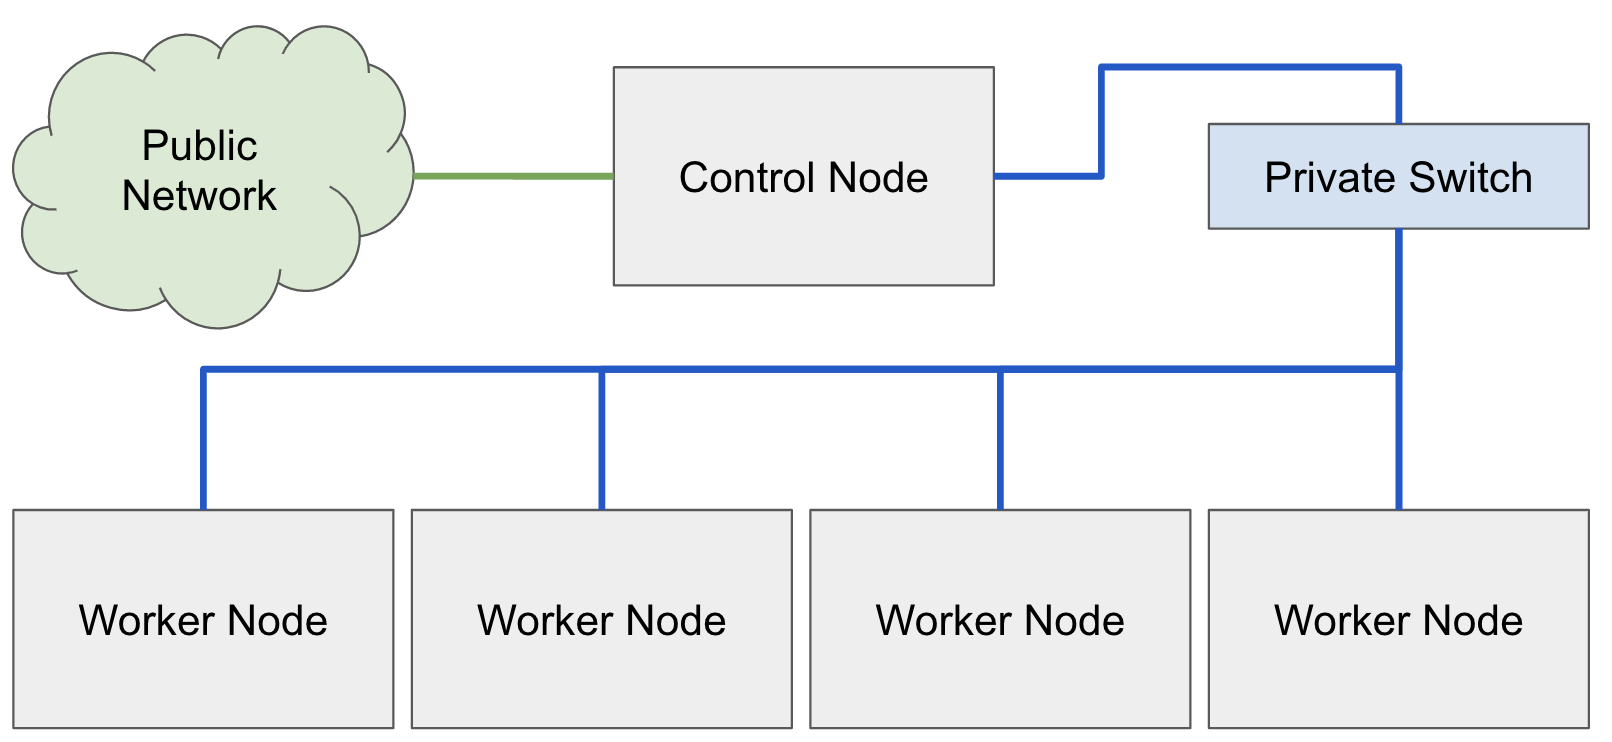
\includegraphics[height=3.5cm]{beowulf_architecture}
\end{frame}
\begin{frame}[fragile]
\frametitle{Warewulf configuration}
\framesubtitle{node images}
\begin{columns}
\column{0.5\textwidth}
\begin{block}{definition}
\begin{itemize}
  \item complete OS images
  \item called containers in warewulf
  \item must be imported from:
  \begin{itemize}
    \item chroot directory
    \item docker registry
    \item local \texttt{dockerd}
  \end{itemize}
  \item several different node images can be imported
  \item node images are vendor independent
\end{itemize}
\end{block}
\column{0.5\textwidth}
\begin{block}{\texttt{registry.suse.com}}
  \begin{itemize}
    \item SUSE SLE 15SP5
  \end{itemize}
\end{block}
\begin{block}{\texttt{registry.opensuse.org}}
  \begin{itemize}
    \item openSUSE Tumleweed
    \item openSUSE Leap 15SP[3-5]
   \end{itemize}
\end{block}
\begin{block}{\texttt{ghcr.io}}
  \begin{itemize}
    \item openSUSE Leap
    \item Rocky EL (8\&9)
    \item Debian Bockworm
  \end{itemize}
\end{block}
\end{columns}
\end{frame}
\begin{frame}[fragile]
\frametitle{Warewulf configuration}
\framesubtitle{node image examples}
\begin{block}{Import the SLE image}
\begin{lstlisting}[style=wwctl]
ww4-host:~> export WAREWULF_OCI_USERNAME=cgoll@suse.com
ww4-host:~> export WAREWULF_OCI_PASSWORD=INTERNAL-USE-ONLY-xxxxxx
ww4-host:~> wwctl container import docker://registry.suse.com/suse/hpc/warewulf4-x86_64/sle-hpc-node:latest sle-hpc
\end{lstlisting}
\end{block}
\begin{block}{Import the Leap image}
\begin{lstlisting}[style=wwctl]
ww4-host:~> wwctl container import docker://registry.opensuse.org/science/warewulf/leap-15.5/containers/kernel:latest leap
\end{lstlisting}
\end{block}
\end{frame}
\begin{frame}[fragile]
\frametitle{Warewulf configuration}
\framesubtitle{node image examples}
\begin{block}{Execute shell in images}
\begin{lstlisting}[style=wwctl]
wwctl container shell sle-hpc
WARN   : Couldn`t mount /etc/SUSEConnect to /etc/SUSEConnect: no such file or directory
WARN   : Couldn`t mount /etc/zypp/credentials.d/SCCcredentials to /etc/zypp/credentials.d/SCCcredentials: no such file or directory
[sle-hpc] Warewulf>
\end{lstlisting}
\begin{itemize}
  \item SLE registration from outer node is mounted into image
\end{itemize}
\end{block}
\end{frame}
\begin{frame}[fragile]
\frametitle{Warewulf configuration}
\framesubtitle{disk management}
\begin{columns}
\column{0.5\textwidth}
\begin{block}{Needs following elements:}
\begin{itemize}
  \item disks
  \item partitions needs parent disk
  \item filesystem needs partent partition
\end{itemize}
\end{block}
\begin{block}{implementation}
  \begin{itemize}
    \item call \texttt{ignition} with {ignition-ww4-disk.service} \\
    \item \textbf{not} in dracut 
    \item \textbf{before} \texttt{sysroot.mount}
  \end{itemize}
\end{block}
\column{0.5\textwidth}
\begin{block}{single parition}
\begin{lstlisting}[style=wwctl]
wwctl node set n01 --diskname /dev/vda --diskwipe --partname scratch --partcreate --fsname scratch --fsformat btrfs --fspath /scratch --fswipe
\end{lstlisting}
\end{block}
\begin{block}{add swap}
\begin{lstlisting}[style=wwctl]
wwctl node set n01 --diskname /dev/vda --partname swap --partsize=1024 --partnumber 1 --fsname swap --fsformat swap --fspath swap
\end{lstlisting}
\end{block}
\end{columns}
\end{frame}
\begin{frame}[fragile]
\frametitle{Warewulf boot}
\framesubtitle{boot process}
\begin{columns}
\column{0.5\textwidth}
\begin{block}{boot with iPXE}
\begin{itemize}
  \item distribution iPXE binaries are used
  \item \texttt{tftp} transfers are small
  \item \texttt{kernel} is extracted from container/node image on the fly
  \item root fs is the container/node image\\
  configuration overlay added on top
  \item \textbf{no} secure boot
\end{itemize}
\end{block}
\column{0.5\textwidth}
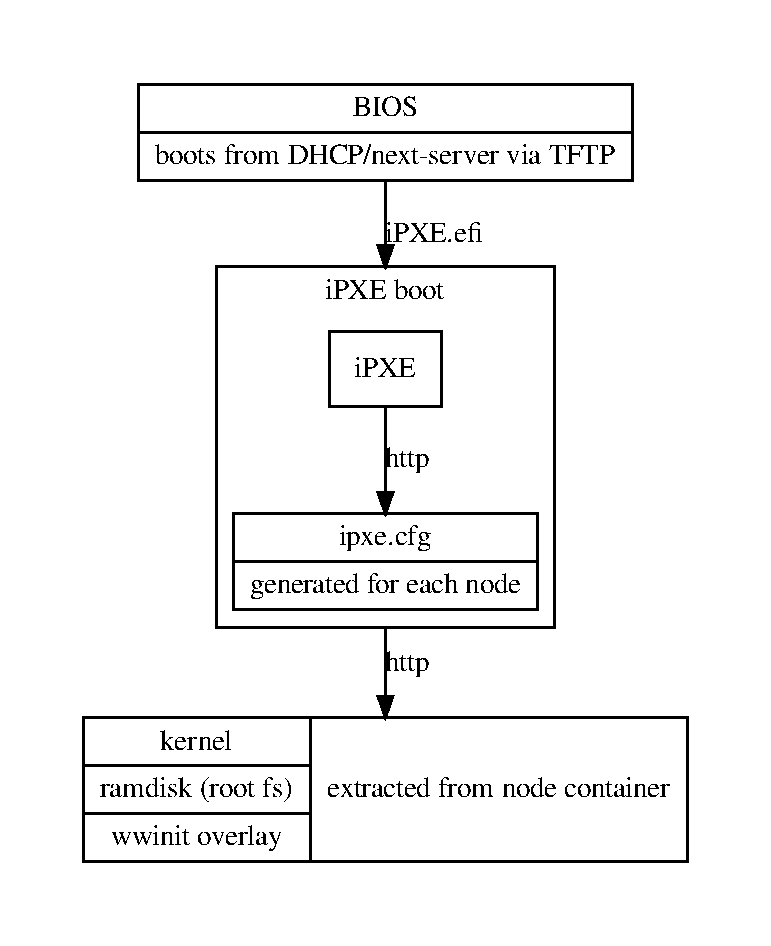
\includegraphics[width=.9\linewidth]{ipxe_boot}
\end{columns}
\end{frame}
\begin{frame}[fragile]
\frametitle{Warewulf boot}
\framesubtitle{boot process}
\begin{columns}
\column{0.5\textwidth}
\begin{block}{boot with grub tftp}
\begin{itemize}
  \item grub \& shim extracted from host
  \item secure boot only possible if host shim \& grub can boot node kernel
\end{itemize}
\end{block}
\column{0.5\textwidth}
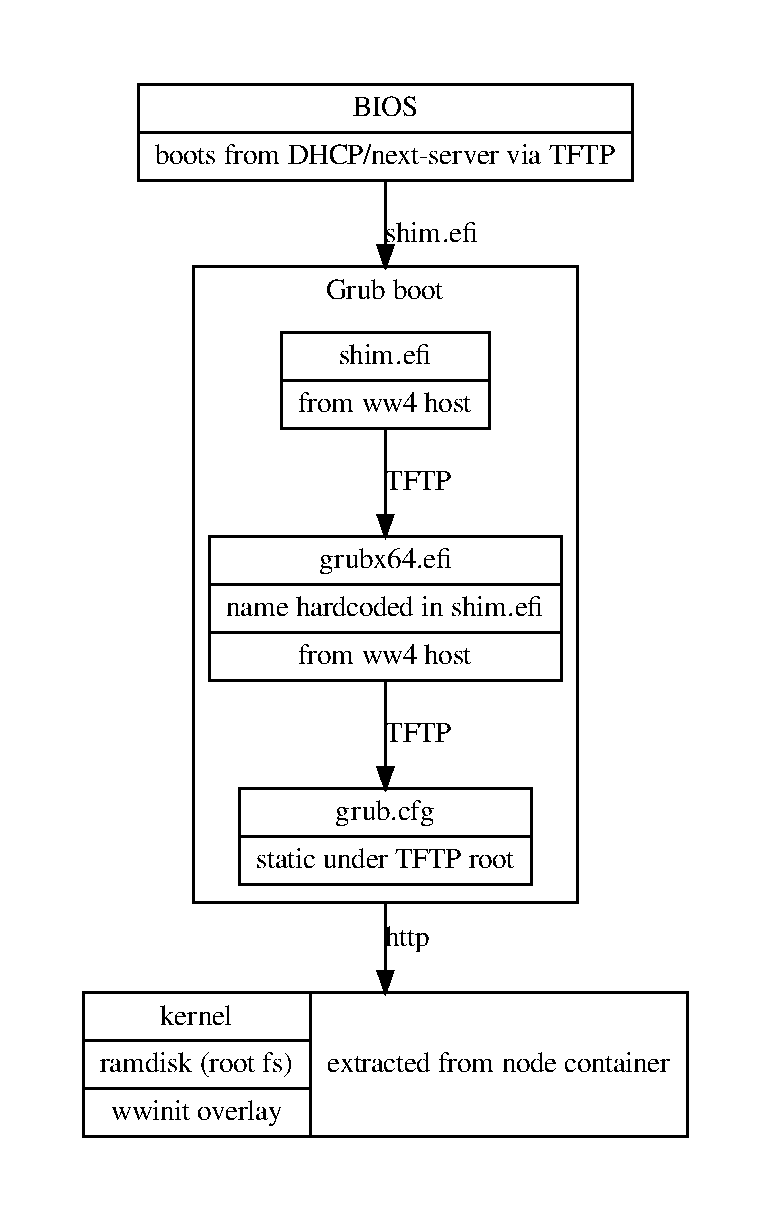
\includegraphics[width=.7\linewidth]{grub_ipxe}
\end{columns}
\end{frame}
\begin{frame}[fragile]
\frametitle{Warewulf boot}
\framesubtitle{boot process}
\begin{columns}
\column{0.5\textwidth}
\begin{block}{boot with grub http}
\begin{itemize}
  \item grub \& shim xtracted from node/container image
  \item secure boot with various distributions
  \item must be configured in BIOS
\end{itemize}
\end{block}
\column{0.5\textwidth}
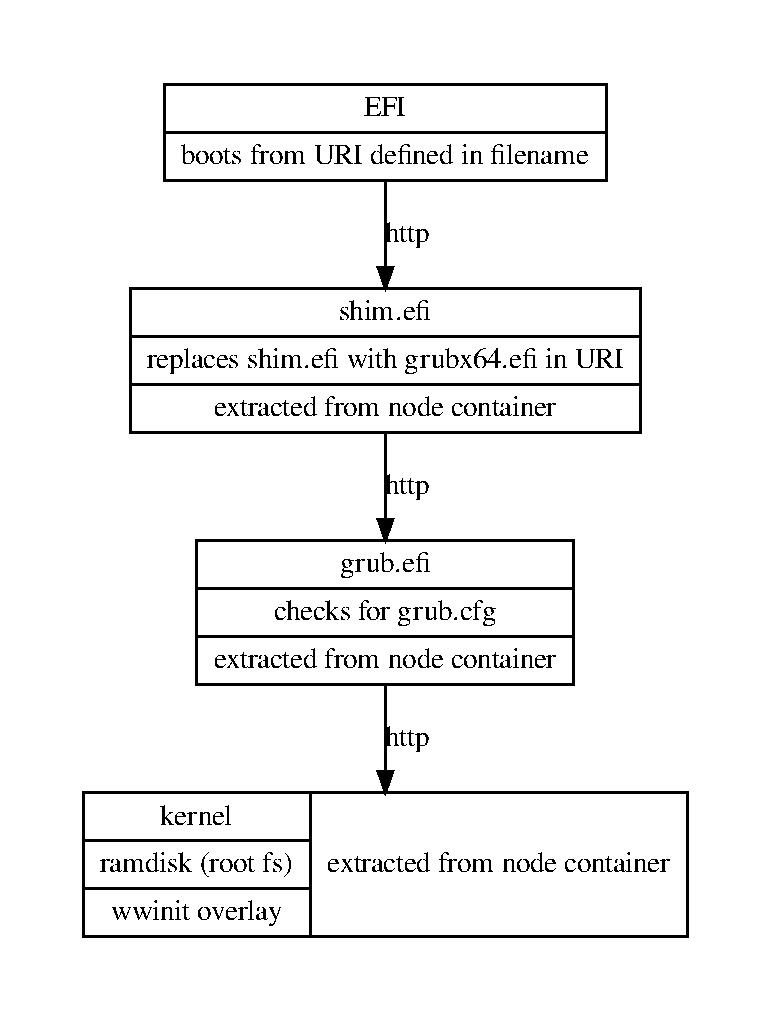
\includegraphics[width=.8\linewidth]{grub_http}
\end{columns}
\end{frame}
\begin{frame}[fragile]
\frametitle{Warewulf}
\framesubtitle{development}
\begin{columns}
\column{0.5\textwidth}
\begin{block}{availiability}
  \begin{itemize}
    \item part of SLE since 15SP5
    \item SLE node/container avaible
  \end{itemize}
\end{block}
\begin{block}{upstream}
\texttt{github.com/warewulf/warewulf} \\
Rocky Linux Foundation project\\
Stakeholders:
\begin{itemize}
  \item SUSE
  \item CIQ
  \item Intel/openHPC
\end{itemize}
\end{block}
\column{0.5\textwidth}

\includegraphics[width=.8\linewidth]{warewulf-logo}
\end{columns}
\end{frame}
\begin{frame}[fragile]
\frametitle{Warewulf}
Thank your, for you attention!
\end{frame}
\end{document}

